% -- Document configuration
\documentclass{article}

% -- Input and language settings
% \usepackage[utf8]{inputenc}
\usepackage[spanish]{babel}
\decimalpoint                             % From babel package to use points instead of commas in decimals

% -- Page and line settings
\usepackage{geometry}
\geometry{letterpaper, 
    % margin=2cm, 
    left=3cm, right=3cm,
    top=1.2cm, bottom=1.2cm,
    includefoot, 
    includehead}
\renewcommand{\baselinestretch}{1.2}

% -- Required packages
\usepackage{xcolor}
\usepackage[many]{tcolorbox}
\usepackage{mathtools,amsfonts,amsmath}     % Loads amsmath if not already loaded
\allowdisplaybreaks                         % To allow page breaks if equations are too long
\usepackage[parfill]{parskip}               % No indent and separation lines for paragraphs
\usepackage{cancel}                         % To cancel math terms
\usepackage[shortlabels]{enumitem}          % To handle enumerations
\usepackage{tikz}
\usetikzlibrary{automata, arrows.meta, positioning}
\usepackage[mode=buildnew]{standalone}      % To import figures in standalone files
\usepackage[hidelinks]{hyperref}
\usepackage[spanish]{cleveref}              % To use autocompleted reference labels, language must be change as in babel package
\usepackage{caption}                        % Caption and subcaption to allow subfigures
\usepackage{subcaption}
\usepackage{float}                          % To specify the location of figures
\usepackage{multicol}                       % To use multicolumns
\usepackage[bottom]{footmisc}               % To locate footnotes at the bottom

% -- Title and heading settings
\usepackage{titling}
\usepackage{fancyhdr}
\pagestyle{fancy}

% -- Code and code formatting
\usepackage{minted}                         % To insert code
\usemintedstyle[julia]{gruvbox-light}       % Code theme and language
\definecolor{bg}{rgb}{0.98, 0.97, 0.88}     % Code block background

\usepackage{fontspec}                       % To allow the use of monospace fonts
\setmonofont{JuliaMono}[Path=./codefonts/, Extension=.ttf, UprightFont=*-Regular, ItalicFont=*-RegularItalic, Scale=0.75]

\usepackage{fancyvrb}                       % To change line number font
\renewcommand{\theFancyVerbLine}{\textcolor{gray}{\footnotesize\texttt{\arabic{FancyVerbLine}}}}

\definecolor{light-gray}{gray}{0.95}        % Color, box and style to show small code thingys inside normal text
\newcommand{\code}[1]{\colorbox{light-gray}{\texttt{#1}}}

% -- Bilbiography preferences
\usepackage[square,numbers]{natbib}
\bibliographystyle{unsrt}

% -- Footnotes without numbering
\newcommand\nnfootnote[1]{%
  \begin{NoHyper}
  \renewcommand\thefootnote{}\footnote{#1}%
  \addtocounter{footnote}{-1}%
  \end{NoHyper}
}

% -- Theorems
\newtheorem{theorem}{Theorem}

\lhead{\theinstitution\ -- \thedepartment}
\chead{}
\rhead{Programación para la IA\ -- \thetitle}
\lfoot{}
\cfoot{\thepage}
\rfoot{}

% -- Problem solution
\newenvironment{solution}
{\begin{quote}
\textbf{Solución:}\medskip

}
{

\hfill\rule{0.5\textwidth}{0.5pt}
\end{quote}}

% -- Equation result
\newcommand{\result}[1]
{
\tcbhighmath[colframe=white, colback=gray!15, sharp corners]
{#1}
}

% -- Function definitions
\newcommand{\dprod}[2]{{#1} \cdot {#2}}
\newcommand{\txtgray}[1]{\textcolor{gray}{#1}}

% -- Author information
\title{Actividad 5}
\author{Leonardo Flores Torres}
\newcommand\theinstitution{Universidad Veracruzana}
\newcommand\thedepartment{Inteligencia Artificial}
\newcommand\thecourse{Programación para la Inteligencia Artificial}

% -- Paths
% \newcommand\codelists{../programs/lists.rkt}

% Remove red color boxes of "syntax errors" in minted
\AtBeginEnvironment{minted}{%
  \renewcommand{\fcolorbox}[4][]{#4}}

% -- Document
\begin{document}

\thispagestyle{empty}

%Title
\begin{center}
\textsc{\theinstitution}\\[2mm]

\thedepartment

\rule{0.6\textwidth}{0.5pt}\\[2mm]

\thecourse \\[4mm]

{\Large \textbf{\thetitle}}\\[2mm]

\theauthor \\[2mm]

{\small \today}
\end{center}
\medskip

% -- 
\vspace{1cm}

Adaptar el algoritmo de Dijkstra para que trabaje en una rejilla donde se defina el punto inicial $(r_i, c_i)$ y el punto final $(r_f, c_f)$ y encuentre la ruta óptima con las siguientes variantes,
\begin{enumerate}
    \item usar 4 vecinos con distancias unitarias,
    \item usar 8 vecinos,
    \item incluir la posibilidad de encontrar obstáculos.
    \begin{solution}
        El módulo desarrollado, \code{ShortestPath}, para resolver esta actividad se muestra en el apéndice de este trabajo. El algoritmo de Dijkstra no fue implementado sino que se utilizó una librería ya desarrollada en \code{julia} que permite el uso de grafos y además incluye la implementación de distintos algoritmos de recorrido y búsqueda de los caminos más cortos, como lo es el de Dijkstra.

        La manera de utilizar el módulo, \code{ShortestPath}, en el \code{REPL} de \code{julia} se muestra a continuación. Primero se define el tamaño de la rejilla en \code{nrows} y \code{ncols}, y con estas variables se computa la representación de índices de los elementos de la rejilla, aunque resulta ser impractica de visualizar mientras más el número más vecinos hay en total dentro de la vecindad.
        \begin{minted}[
            frame=none,
            autogobble,
            obeytabs=false,
            breaklines,
            tabsize=4,
            linenos=true,
            % numbersep=-10pt,
            baselinestretch=1,
            firstnumber=1,
            bgcolor=bg!70,
            ]{julia}
            julia> nrows = 40; ncols = 40;

            julia> idarray = [i for i in 1:(ncols * nrows)] |> x -> reshape(x, ncols, nrows) |> transpose;

            julia> start = [10, 3]; finish = [35, 37];
        \end{minted}

        Una vecindad es el nombre dado a la rejilla tomando en cuenta los puntos libres por los que se puede transitar, y los obstáculos, que son puntos imposibles de alcanzar. Además, los obstáculos se eligen de pixeles de manera aleatoria de la rejilla inicialmente libre, esto quiere decir que todos los pixeles son alzancables al inicio, se hace un muestreo aleatorio y aquellos elegidos cambian su estado a obstáculos. El argumento \code{obsdensity} de la función \code{neighborhood} indica la densidad de obstáculos deseada entre $[0, 1]$. 

        Se computó una vecindad con los puntos de partida inicial y final mostrados en \code{start} y \code{finish}, respectivamente, y una densidad de obstáculos del $0.25$. También se hizo una copia profunda de la vecindad \code{nh} en \code{nhdiag} ya que se obtuvieron las matrices de adyacencia para los casos donde el movimiento se puede dar sin y con diagonales en la misma rejilla, para 4 y 8 vecinos, respectivamente.
        \begin{minted}[
            frame=none,
            autogobble,
            obeytabs=false,
            breaklines,
            tabsize=4,
            linenos=true,
            % numbersep=-10pt,
            baselinestretch=1,
            firstnumber=last,
            bgcolor=bg!70,
            ]{julia}
            julia> nh, obs = sp.neighborhood(nrows, ncols; start=start, finish=finish, obsdensity=0.25); sp.visualize(nh)

            julia> nhdiag = deepcopy(nh);

            julia> adjmat = sp.adjacencyMatrix(nrows, ncols; obstacles=obs, allowdiags=false);

            julia> adjmatdiag = sp.adjacencyMatrix(nrows, ncols; obstacles=obs, allowdiags=true);
        \end{minted}

        Las matrices de adyacencia guardadas en las variables \code{adjmat} y \code{adjmatdiag} requieren como argumentos la lista de obstaculos en \code{obstacles}, si las diagonales son permitidas o no en \code{allowdiags}, y el número de filas y de columnas. Estos dos primeros argumentos son posicionales mientras que los primeros dos mencionados son argumentos de palabra clave, se observa la división entre un tipo de argumentos y otro con un \code{;} dentro de los argumentos de una función.

        Posteriormente se obtienen los caminos y las distancias de esos caminos con la función \code{findPath}; se computaron los caminos sin diagonales en \code{path} y con diagonales en \code{pathdiag}, con sus repectivas matrices de adyacencia. Para terminar, los caminos se usan para cambiar el estado de los pixeles en las vecindades \code{nh} y \code{nhdiag} con la función \code{updateneighborhood!}. Nótese que la función lleva un signo de admiración \code{!} al final de su nombre para denotar que es una función que modifica alguno de sus argumentos.
        \begin{minted}[
            frame=none,
            autogobble,
            obeytabs=false,
            breaklines,
            tabsize=4,
            linenos=true,
            % numbersep=-10pt,
            baselinestretch=1,
            firstnumber=last,
            bgcolor=bg!70,
            ]{julia}
            julia> path, dist = sp.findPath(adjmat, ncols; start=start, finish=finish);

            julia> pathdiag, distdiag = sp.findPath(adjmatdiag, ncols; start=start, finish=finish);

            julia> sp.updateneighborhood!(nhdiag, pathdiag); sp.visualize(nhdiag)

            julia> sp.updateneighborhood!(nh, path); sp.visualize(nh)

            julia> dist
            59.0

            julia> distdiag
            46.11269837220809
        \end{minted}

        En la \cref{fig:rejilla_40x40} se muestran las imágenes para una rejilla de $40 \times 40$ incluyendo el caso en que el movimiento hacia vecinos solamente se da horizontal y verticalmente, \cref{fig:nodiags_obs_25percent_40x40}, y el caso en que el movimiento diagonal está permitido, \cref{fig:diags_obs_25percent_40x40}. Las distancias del recorrido en cada una de ellas son de $50$ unidades sin diagonales en la \cref{fig:nodiags_obs_25percent_40x40}, y de $46.11$ unidades considerando diagonales en la \cref{fig:diags_obs_25percent_40x40}.
        \begin{figure}[ht!]
            \centering
            \begin{subfigure}{0.4\textwidth}
                \centering
                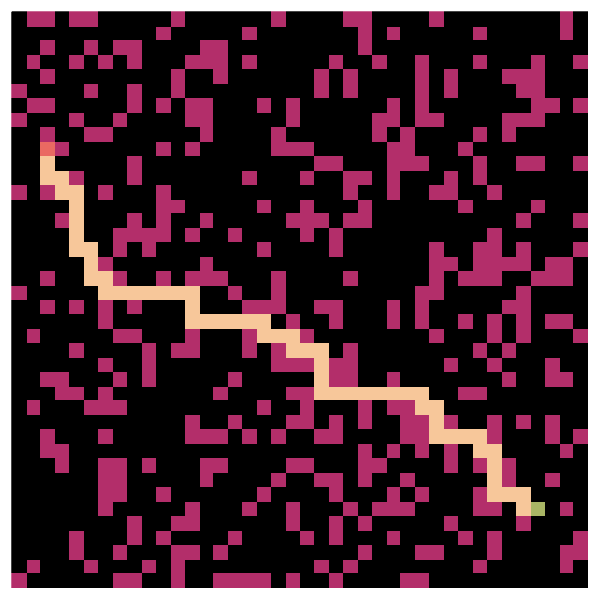
\includegraphics[scale=0.3]{../figures/path_01.png}
                \caption{4 vecinos (diagonales no permitidas); $\text{distancia} = 59 u$.}
                \label{fig:nodiags_obs_25percent_40x40}
            \end{subfigure}
            \hspace{1cm}
            %
            \begin{subfigure}{0.4\textwidth}
                \centering
                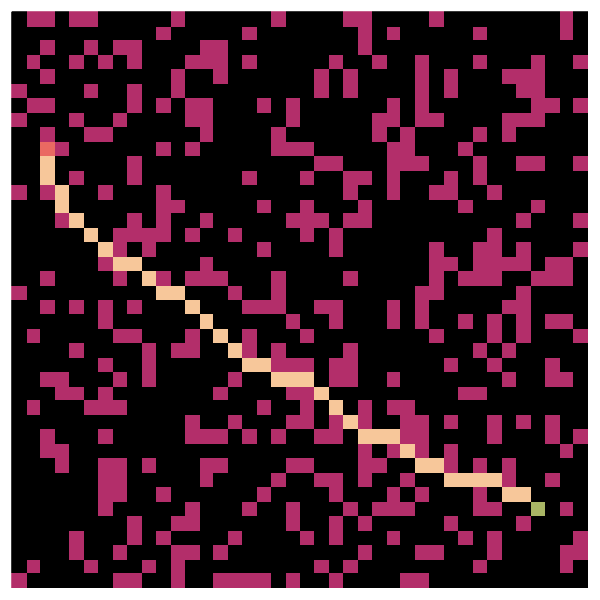
\includegraphics[scale=0.3]{../figures/path_01_diag.png}
                \caption{8 vecinos (diagonales permitidas); $\text{distancia} = 46.1126 u$.}
                \label{fig:diags_obs_25percent_40x40}
            \end{subfigure}
            \caption{Rejilla de $40 \times 40$ con obstaculos al $25\%$.}
            \label{fig:rejilla_40x40}
        \end{figure}

        Los pixeles mostrados en color \fcolorbox{black}{black}{\rule{0pt}{4pt}\rule{4pt}{0pt}} son los pixeles libres por los que se puede transitar mientras que los mostrados de color los pixeles de color \fcolorbox{black}{obstacle}{\rule{0pt}{4pt}\rule{4pt}{0pt}} son los obstáculos; el pixel de color \fcolorbox{black}{start}{\rule{0pt}{4pt}\rule{4pt}{0pt}} es el punto de partida definido en \code{start}, el pixel de color \fcolorbox{black}{finish}{\rule{0pt}{4pt}\rule{4pt}{0pt}} es el punto de llegada definido en \code{finish}, y los pixeles de color \fcolorbox{black}{path}{\rule{0pt}{4pt}\rule{4pt}{0pt}} muestran el camino atravesado para llegar a la meta.

        Esta implementación permite utilizar dimensiones para la rejilla diferentes de $n \times n$, esto quiere decir que se pueden elegir un número diferente de filas que de columnas, y viceversa. Un ejemplo de esto se muestra en la \cref{fig:rejilla_20x35}, con 20 filas y 35 columnas. El camino sin diagonales permitidas es de 50 unidades, mientras que aquel en que se permiten las diagonales tiene longitud de 36.87 unidades.
        \begin{figure}[ht!]
            \centering
            \begin{subfigure}{0.4\textwidth}
                \centering
                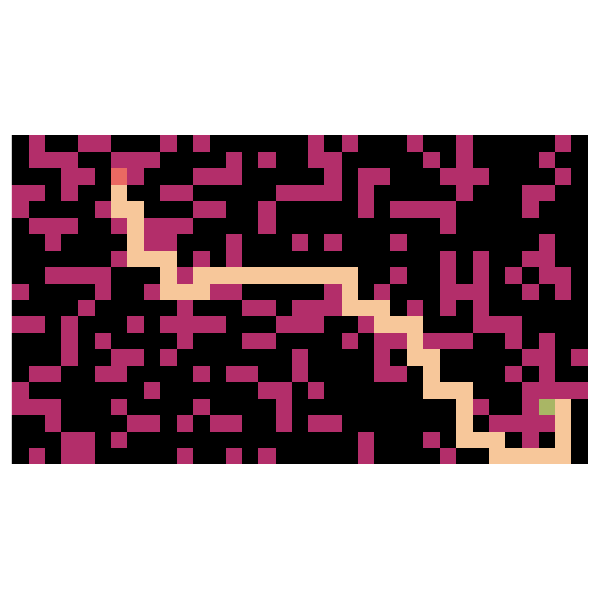
\includegraphics[scale=0.3]{../figures/path_02.png}
                \caption{4 vecinos (diagonales no permitidas); $\text{distancia} = 50 u$.}
            \end{subfigure}
            \hspace{1cm}
            %
            \begin{subfigure}{0.4\textwidth}
                \centering
                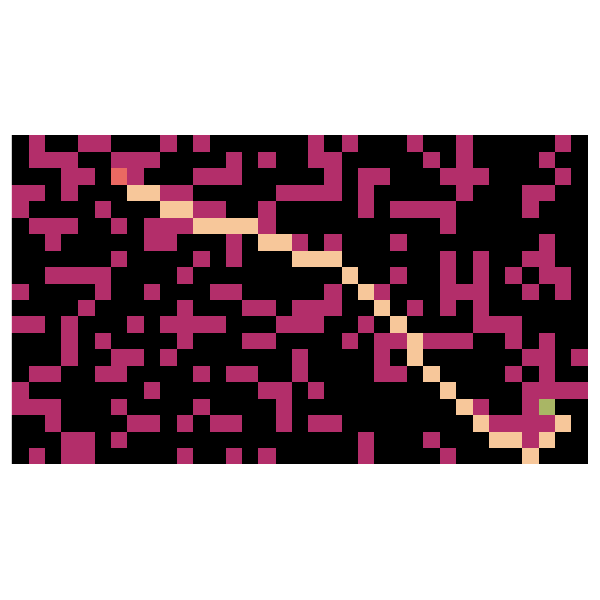
\includegraphics[scale=0.3]{../figures/path_02_diag.png}
                \caption{8 vecinos (diagonales no permitidas); $\text{distancia} = 36.87 u$.}
            \end{subfigure}
            \caption{Rejilla de $20 \times 35$ con obstáculos del $30\%$.}
            \label{fig:rejilla_20x35}
        \end{figure}

        Por completez quisiera explicar la manera en como se computa la matriz de adyacencia, necesaria para pasarla como argumento a las funciones que se encargan de las operaciones para grafos. El problema se reduce a tener una rejilla de la forma 
        
    \end{solution}
\end{enumerate}

\clearpage
\section*{Apéndice}
\inputminted[
    frame=none,
    autogobble,
    obeytabs=false,
    breaklines,
    tabsize=4,
    linenos=true,
    % numbersep=-10pt,
    baselinestretch=1,
    firstnumber=1,
    bgcolor=bg!70,]{julia}{\codepath}

\nocite{*} % to call all references even if they are not cited in the text
\bibliography{references.bib}

\end{document}